\documentclass{standalone}

\usepackage{ tikz }
\usetikzlibrary{automata, positioning, arrows}

\tikzset{->, >=stealth, node distance=3cm, every state/.style={thick, fill=gray!10}, initial text=$ $, every edge/.append style={font=\tiny}
}

\begin{document}
    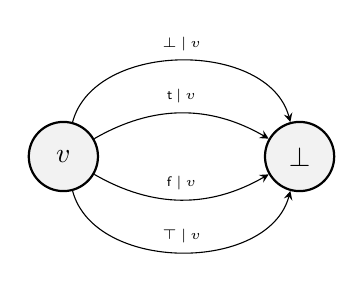
\begin{tikzpicture}
        \node[state] (v) {$v$};
        \node[state, right of=v] (bot) {$\bot$};

        \draw (v) edge[bend left, above] node{$ \mathsf{t} \,|\, v$} (bot)
              (v) edge[bend right, above] node {$ \mathsf{f} \,|\, v$} (bot)
              (v) edge[bend right=75, above] node{$ \top \,|\, v$} (bot)
              (v) edge[bend left=75, above] node{$ \bot \,|\, v$} (bot)
        ;
    \end{tikzpicture}
\end{document}